%%%%%%%%%%%%%%%%%%%%%%%%%%%%%%%%%%%%%%%%%
% Jacobs Landscape Poster
% LaTeX Template
% Version 1.1 (14/06/14)
%
% Created by:
% Computational Physics and Biophysics Group, Jacobs University
% https://teamwork.jacobs-university.de:8443/confluence/display/CoPandBiG/LaTeX+Poster
%
% Further modified by:
% Nathaniel Johnston (nathaniel@njohnston.ca)
%
% This template has been downloaded from:
% http://www.LaTeXTemplates.com
%
% License:
% CC BY-NC-SA 3.0 (http://creativecommons.org/licenses/by-nc-sa/3.0/)
%
%%%%%%%%%%%%%%%%%%%%%%%%%%%%%%%%%%%%%%%%%

%----------------------------------------------------------------------------------------
%	PACKAGES AND OTHER DOCUMENT CONFIGURATIONS
%----------------------------------------------------------------------------------------

\documentclass[final]{beamer}

\usepackage[scale=0.8]{beamerposter} % Use the beamerposter package for laying out the poster

\usetheme{confposter} % Use the confposter theme supplied with this template

\setbeamercolor{block title}{fg=ngreen,bg=white} % Colors of the block titles
\setbeamercolor{block body}{fg=black,bg=white} % Colors of the body of blocks
\setbeamercolor{block alerted title}{fg=white,bg=dblue!70} % Colors of the highlighted block titles
\setbeamercolor{block alerted body}{fg=black,bg=dblue!10} % Colors of the body of highlighted blocks
% Many more colors are available for use in beamerthemeconfposter.sty

%-----------------------------------------------------------
% Define the column widths and overall poster size
% To set effective sepwid, onecolwid and twocolwid values, first choose how many columns you want and how much separation you want between columns
% In this template, the separation width chosen is 0.024 of the paper width and a 4-column layout
% onecolwid should therefore be (1-(# of columns+1)*sepwid)/# of columns e.g. (1-(4+1)*0.024)/4 = 0.22
% Set twocolwid to be (2*onecolwid)+sepwid = 0.464
% Set threecolwid to be (3*onecolwid)+2*sepwid = 0.708

\newlength{\sepwid}
\newlength{\onecolwid}
\newlength{\twocolwid}
\newlength{\threecolwid}
\setlength{\paperwidth}{36in} % A0 width: 46.8in
\setlength{\paperheight}{24in} % A0 height: 33.1in
\setlength{\sepwid}{0.024\paperwidth} % Separation width (white space) between columns
\setlength{\onecolwid}{0.22\paperwidth} % Width of one column
\setlength{\twocolwid}{0.464\paperwidth} % Width of two columns
\setlength{\threecolwid}{0.708\paperwidth} % Width of three columns
\setlength{\topmargin}{-0.5in} % Reduce the top margin size
%-----------------------------------------------------------

\usepackage{graphicx}  % Required for including images
\graphicspath{ {./img/} }
\usepackage{booktabs,multicol} % Top and bottom rules for tables

%----------------------------------------------------------------------------------------
%	TITLE SECTION
%----------------------------------------------------------------------------------------


\title{\textit{ColorUNet}: A convolutional classification approach to colorization} % Poster title

\author{Vincent Billaut, Matthieu de Rochemonteix, Marc Thibault} % Author(s)

\institute{CS231n Final Project, 03/12/2018} % Institution(s)

%----------------------------------------------------------------------------------------

\begin{document}

\small
\addtobeamertemplate{block end}{}{\vspace*{2ex}} % White space under blocks
\addtobeamertemplate{block alerted end}{}{\vspace*{2ex}} % White space under highlighted (alert) blocks

\setlength{\belowcaptionskip}{2ex} % White space under figures
\setlength\belowdisplayshortskip{2ex} % White space under equations

\begin{frame}[t] % The whole poster is enclosed in one beamer frame

\begin{columns}[t] % The whole poster consists of three major columns, the second of which is split into two columns twice - the [t] option aligns each column's content to the top

\begin{column}{\sepwid}\end{column} % Empty spacer column

\begin{column}{\onecolwid} % The first column

%----------------------------------------------------------------------------------------
%	OBJECTIVES
%----------------------------------------------------------------------------------------

\begin{alertblock}{Objectives}

\begin{itemize}
\item Implementation of a lightweight version of \cite{zhang2016colorful}
\item Implementation of an architecture from scratch
\item Extension to videos.
\end{itemize}

\end{alertblock}

%----------------------------------------------------------------------------------------
%	INTRODUCTION
%----------------------------------------------------------------------------------------

\begin{block}{Colorization as classification}

  \begin{figure}
  \begin{center}
  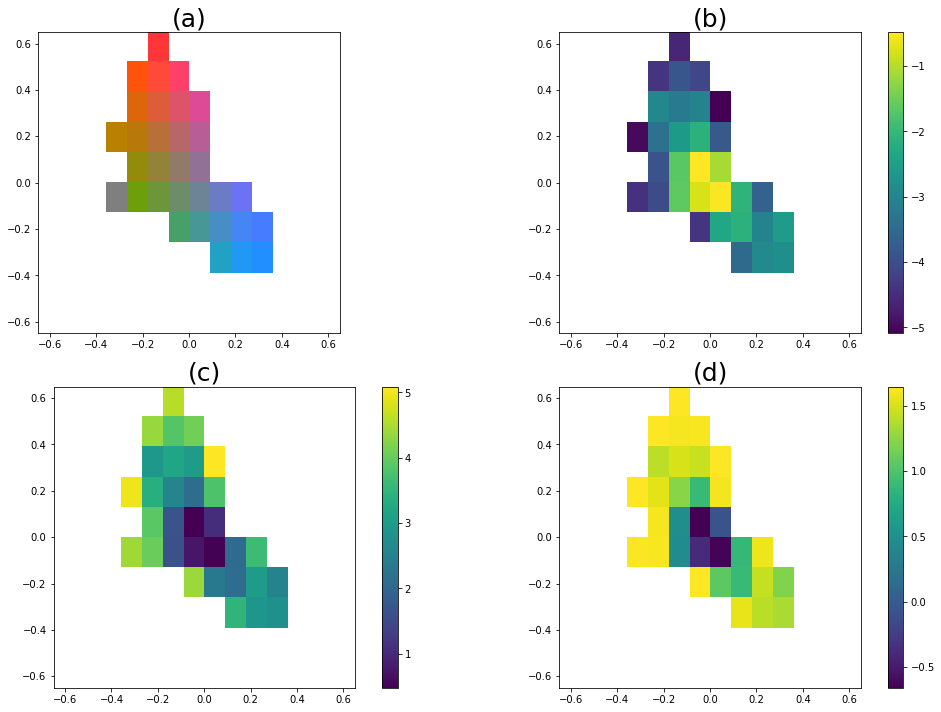
\includegraphics[width=.5\linewidth]{cdexample}\label{colormap}
  \caption{ (a) Color map, showing the mean color (\textit{chrominance}) of each of the selected bins (32 bins to select). (b) Frequency map (log-scale), shows the empirical frequency of the colors within each bin. (c) Inverse-frequency map. (d) Weight map (log-scale), shows the weights assigned to each bin after rebalancing.}
  \end{center}
  \end{figure}

We approach the colorization problem as a \textbf{classification problem}. The main purpose is to boost the possibility of a rare color being predicted, and therefore we use the following tricks:
\begin{itemize}
\item Use \textit{rebalancing} to give larger weights to rare colors in our loss function.
\item Use an \textit{annealed-mean} to output predictions $y$ from the probability distribution $\textbf{Z}$ over our $n$ bins to the full original color space. To achieve this we use a temperature parameter $T > 0$ in the following softmax-like formula for one pixel $$y = f_T(\textbf{z}) = {\exp(\log(\textbf{z}) / T) \over \sum_i \exp(\log(\textbf{z}_i) / T)}$$ where $\textbf{z}$ is the $n$-dimensional probability vector of a given pixel over the $n$ bins, and the sum in the denominator is over all the bins.
\end{itemize}




\end{block}

%------------------------------------------------
\begin{block}{Dataset}

To train our model, we used subsets of the SUN and ImageNet datasets. We selected 8 categories from ImageNet and 14 categories from SUN, that correspond mainly to nature landscapes. Our final training set is composed of 13,469 images, downscaled to a $256\times 256$ resolution.

We used data augmentation to increase the robustness of training, namely :
\begin{itemize}
\item Flipping the image along the horizontal axis;
\item Adding noise to the image (with different intensities);
\item Selecting random crops of the image.
\end{itemize}
This procedure increases the size of the dataset sevenfold
\end{block}



\end{column} % End of the first column




\begin{column}{\sepwid}\end{column} % Empty spacer column


\begin{column}{\twocolwid} % Begin a column which is two columns wide (column 2)

  \begin{block}{ColorUNet outputs: influence of temperature}

  \begin{figure}
  \begin{center}
  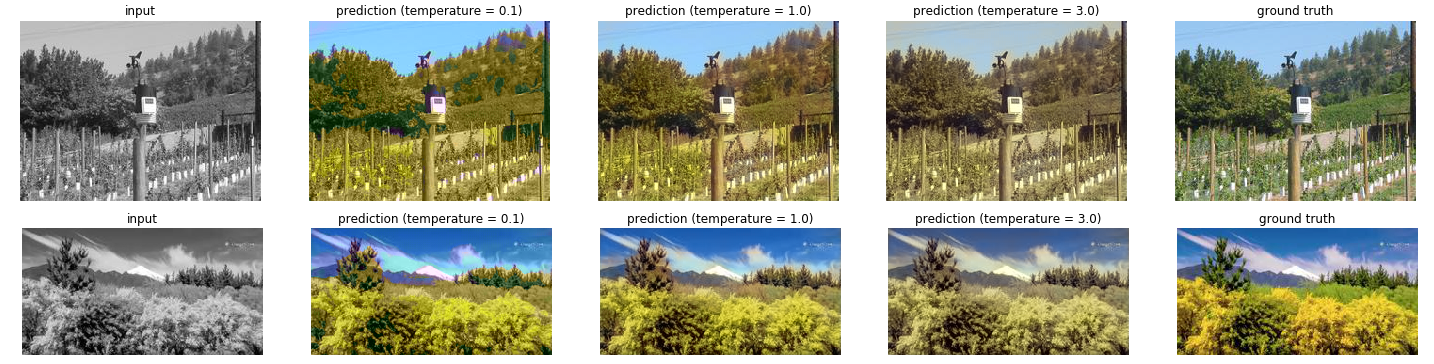
\includegraphics[width=.8\twocolwid]{img/good_cropped.png}
  \caption{Examples of images colorized by ColorUNet. Temperature enables a trade-off between vivid colors and conservative colorizing.}
  \label{good}
  \end{center}
  \end{figure}

  \begin{figure}
  \begin{center}
  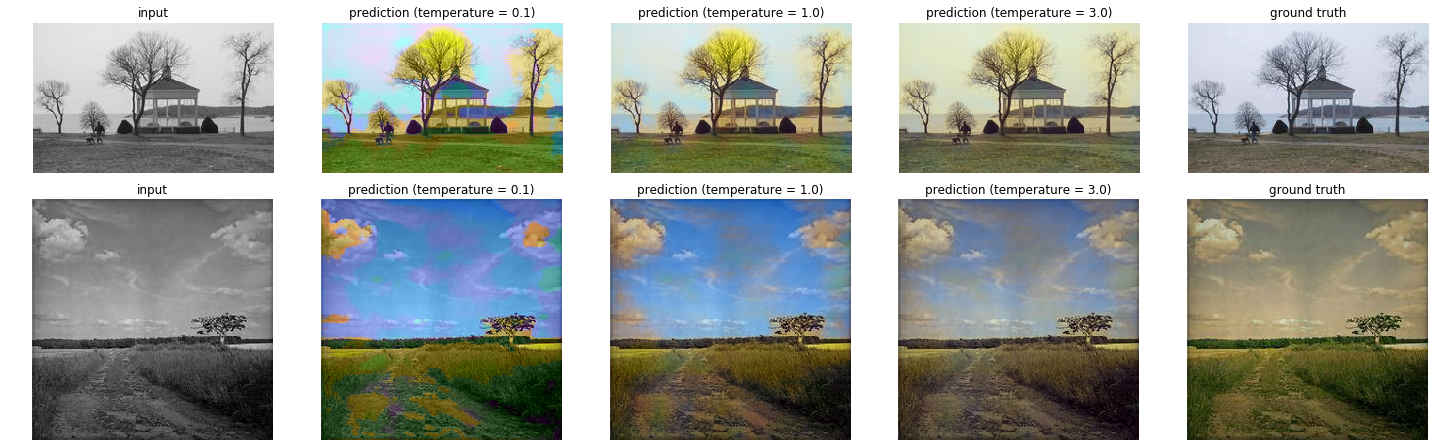
\includegraphics[width=.8\twocolwid]{img/better_cropped}
  \caption{Sample predictions of the ColorUNet on the validation set, for bland input images. The ColorUNet’s output is more colorful than the ground truth. The bottom example is an old photograph with weared tones.}
  \label{better}
  \end{center}
  \end{figure}

  \end{block}

  \begin{columns}[t,totalwidth=.7\twocolwid] % Split up the two columns wide column again
    \begin{column}{.075\twocolwid}\end{column}
    \begin{column}{.85\twocolwid}

    \begin{alertblock}{Understand ColorUNet: Confidence maps}

    \begin{figure}
    \begin{center}
    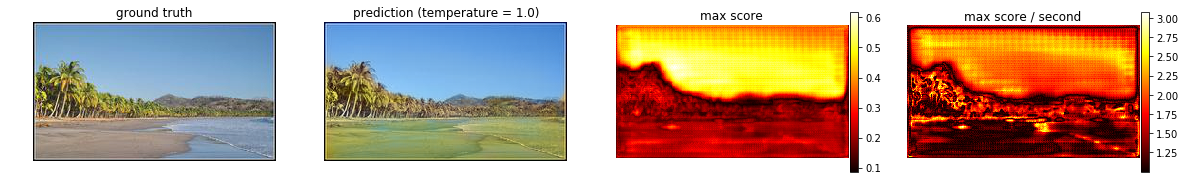
\includegraphics[width=.6\twocolwid]{img/confidence}
    \caption{Confidence maps for the colorization of an image.}
    \label{confidence}
    \end{center}
    \end{figure}

    The model outputs a probability distribution for each pixel, $(p_i)_{i=1...32}$

    Confidence maps are defined, for each pixel, as
    $C_1 = p_{(1)}\ \ \ \ \ \ \ \  C_2 = \frac{p_{(1)}}{p_{(2)}}$
    \end{alertblock}

    \end{column}
    \begin{column}{.075\twocolwid}\end{column}
  \end{columns}


% %----------------------------------------------------------------------------------------
% %	IMPORTANT RESULT
% %----------------------------------------------------------------------------------------

%\begin{alertblock}{Important Result}
%
%Lorem ipsum dolor \textbf{sit amet}, consectetur adipiscing elit. Sed commodo molestie porta. Sed ultrices scelerisque sapien ac commodo. Donec ut volutpat elit.
%
%\end{alertblock}

%----------------------------------------------------------------------------------------

\begin{columns}[t,totalwidth=\twocolwid] % Split up the two columns wide column again

\begin{column}{\onecolwid} % The first column within column 2 (column 2.1)

%----------------------------------------------------------------------------------------
%	MATHEMATICAL SECTION
%----------------------------------------------------------------------------------------
\begin{block}{}
These results have been obtained using NVIDIA K80 GPUs. Total training time was roughly 10 hours. Batch size used is 64.

\end{block}

%----------------------------------------------------------------------------------------

\end{column} % End of column 2.1

\begin{column}{\onecolwid} % The second column within column 2 (column 2.2)

%----------------------------------------------------------------------------------------
%	RESULTS
%----------------------------------------------------------------------------------------
\begin{block}{}
{\footnotesize
\bibliographystyle{ieee}
\bibliography{references}
}
\end{block}


%----------------------------------------------------------------------------------------

\end{column} % End of column 2.2


\end{columns} % End of the split of column 2

\end{column} % End of the second column

\begin{column}{\sepwid}\end{column} % Empty spacer column

\begin{column}{\onecolwid} % The third column

%----------------------------------------------------------------------------------------
%	CONCLUSION
%----------------------------------------------------------------------------------------

\begin{block}{Model architecture}

  \begin{figure}
  \begin{center}
  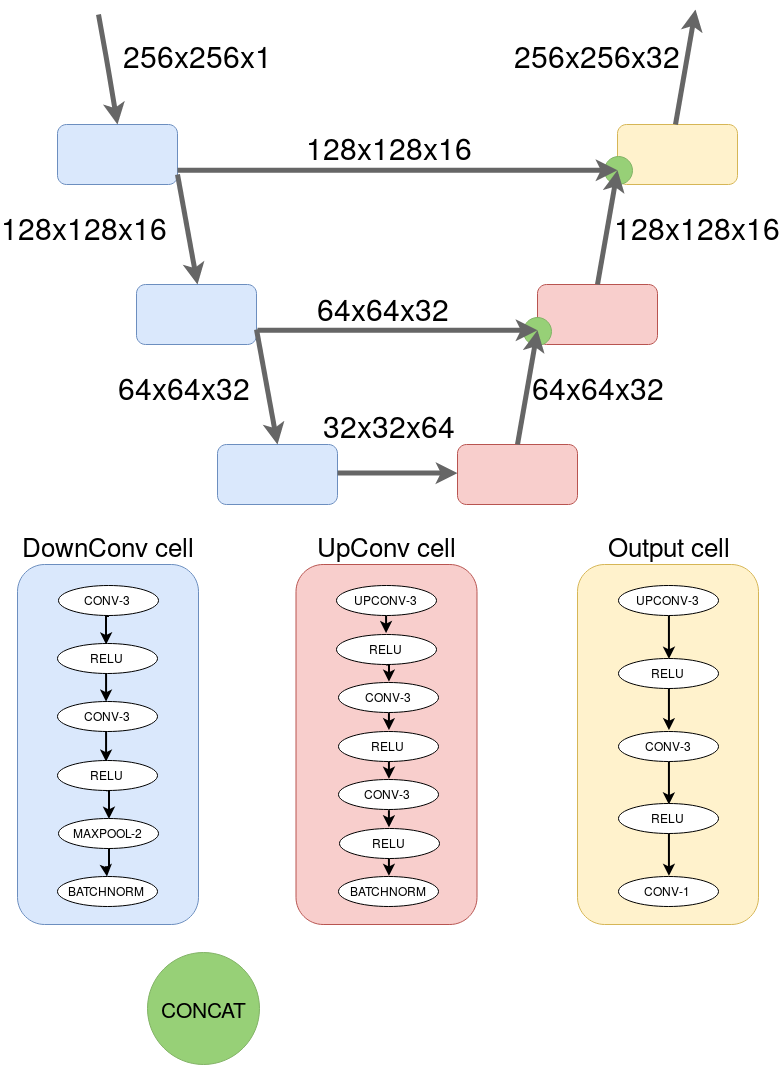
\includegraphics[width=.5\linewidth]{diagram}
  \caption{Structure of the ColorUNet.}
  \label{structure}
  \end{center}
  \end{figure}

After trying a simple convolutional architecture and a deep bottleneck architecture, we implemented an architecture based on the approach of \cite{ronneberger2015unet}, to improve both the gradient flow and the upscaling process.

\end{block}

%----------------------------------------------------------------------------------------
%	ADDITIONAL INFORMATION
%----------------------------------------------------------------------------------------

% \begin{block}{Additional Information}

% Maecenas ultricies feugiat velit non mattis. Fusce tempus arcu id ligula varius dictum.
% \begin{itemize}
% \item Curabitur pellentesque dignissim
% \item Eu facilisis est tempus quis
% \item Duis porta consequat lorem
% \end{itemize}

% \end{block}

%----------------------------------------------------------------------------------------
%	REFERENCES
%----------------------------------------------------------------------------------------

\begin{block}{Results analysis}


\begin{figure}
\begin{center}
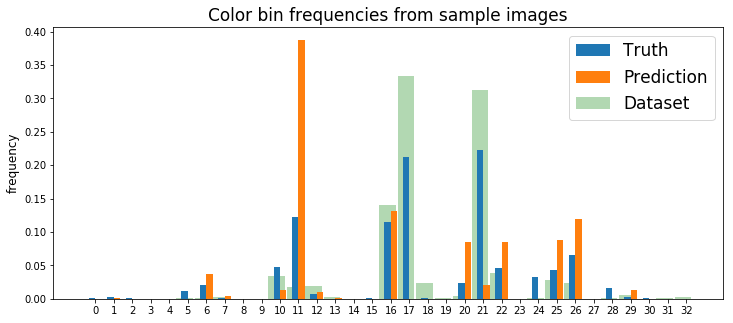
\includegraphics[width=\linewidth]{histogram_compact}
\caption{Histograms of the frequencies of the 32 selected color bins.}
\label{histogram}
\end{center}
\end{figure}



\end{block}

\begin{block}{Comparison to baseline}

Insert output + zhang here

\end{block}

%----------------------------------------------------------------------------------------
%	ACKNOWLEDGEMENTS
%----------------------------------------------------------------------------------------

% \setbeamercolor{block title}{fg=red,bg=white} % Change the block title color

% \begin{block}{Acknowledgements}

% \small{\rmfamily{Nam mollis tristique neque eu luctus. Suspendisse rutrum congue nisi sed convallis. Aenean id neque dolor. Pellentesque habitant morbi tristique senectus et netus et malesuada fames ac turpis egestas.}} \\

% \end{block}

%----------------------------------------------------------------------------------------
%	CONTACT INFORMATION
%----------------------------------------------------------------------------------------

% \setbeamercolor{block alerted title}{fg=black,bg=norange} % Change the alert block title colors
% \setbeamercolor{block alerted body}{fg=black,bg=white} % Change the alert block body colors

% \begin{alertblock}{Contact Information}

% \begin{itemize}
% \item Web: \href{http://www.university.edu/smithlab}{http://www.university.edu/smithlab}
% \item Email: \href{mailto:john@smith.com}{john@smith.com}
% \item Phone: +1 (000) 111 1111
% \end{itemize}

% \end{alertblock}

% \begin{center}
% \begin{tabular}{ccc}
% \includegraphics[width=0.4\linewidth]{logo.png} & \hfill & \includegraphics[width=0.4\linewidth]{logo.png}
% \end{tabular}
% \end{center}

%----------------------------------------------------------------------------------------

\end{column} % End of the third column

\end{columns} % End of all the columns in the poster

\end{frame} % End of the enclosing frame


\end{document}
